\chapter{Resultados e Discussão}\label{cap:resultados}

Para a definição da proposta deste projeto, realizaram-se entrevistas com uma equipe multidisciplinar de profissionais de saúde, atuante na Confederação Nacional das Cooperativas Médicas (UNIMED) - Centro Oeste e Tocantins, a qual é composta por uma psicóloga, uma terapeuta ocupacional e uma fonoaudióloga. As profissionais apresentaram alguns tipos de pacientes e patologias, sendo que o foco voltou-se para o tratamento do transtorno do espectro autista (TEA). Assim sendo, a equipe elicitou algumas técnicas utilizadas no tratamento desse tipo de transtorno. Foram elas: PECS; ABA e TEACCH, as quais podem ser melhor entendidas na seção \ref{tratamentos}. Com base no estudo dessas técnicas de tratamento, surgiu a oportunidade de desenvolver um projeto de um aplicativo para dispositivos móveis para auxiliar o profissional no tratamento de crianças com transtorno do espectro autista, utilizando técnicas de e-learning e gamificação. 

\section{Técnicas/Mecânicas da Gamificação}
Definiu-se como público alvo do aplicativo: os profissionais de saúde que atuam nesse tipo de tratamento; os pacientes diagnosticados com TEA, com grau leve e moderado, e idades variando entre 5 e 10 anos; e os pais ou responsáveis pelos pacientes.

Realizou-se um levantamento das mecânicas de gamificação, citadas por \citeonline{zichermann2011gamification}, as quais foram avaliadas e classificadas em relação a qual público elas se aplicariam de melhor maneira. Chegou-se a seguinte tabela:
\begin{table}[h]
	\centering
	\caption{Relação de Mecânicas de Gamificação por Atores do Sistema}
	\label{mecPorAlvo}
	\begin{tabular}{llll}
		\hline
		\textbf{Mecânicas}     & \textbf{Paciente}     & \textbf{Responsável}  & \textbf{Profissional} \\ \hline
		\textbf{Pontos}        &                       & \multicolumn{1}{c}{X} & \multicolumn{1}{c}{X} \\
		\textbf{Níveis}        &                       & \multicolumn{1}{c}{X} & \multicolumn{1}{c}{X} \\
		\textbf{Classificação} &                       &                       & \multicolumn{1}{c}{X} \\
		\textbf{Emblemas}      & \multicolumn{1}{c}{X} &                       &                       \\
		\textbf{Desafios}      &                       & \multicolumn{1}{c}{X} &                       \\
		\textbf{Integração}    & \multicolumn{1}{c}{X} &                       &                       \\
		\textbf{Engajamento}   & \multicolumn{1}{c}{X} &                       &                       \\ \hline
	\end{tabular}
\end{table}


A Tabela \ref{mecPorAlvo} indica quais mecânicas estarão disponíveis para cada um dos públicos alvos, e essa mecânica é a responsável pela manutenção do interesse dos usuários no aplicativo gamificado. A seguir, são descritas as técnicas de gamificação e a relação com cada usuário do sistema:

	\begin{itemize}
	\item Mecânicas relacionadas aos pacientes
		\subitem1 - Emblema: os emblemas serve como forma de motivar o paciente a participar das sessões, sendo que estes serão conquistados com a participação e conclusão das atividades que forem atribuídas. Os emblemas são algo atraente ao paciente, sendo efetivo no ato de motivar e querer se envolver no uso da aplicação.
		
		\begin{figure}[H]
			\centering
			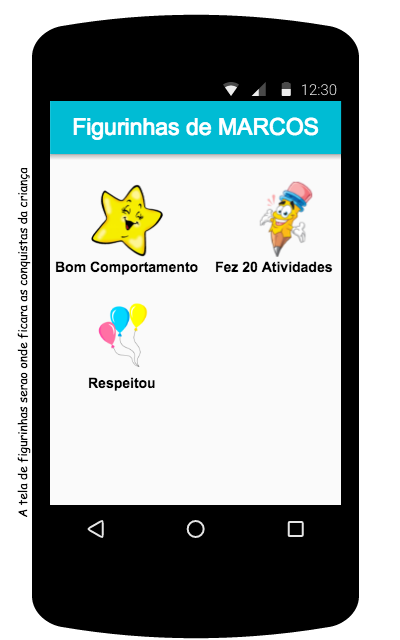
\includegraphics[scale=0.6]{img/emblemaspaciente.png}
			\caption{Protótipo da Tela de Emblemas}
			Fonte:Autor, 2018
			\label{emblemas}
		\end{figure}
		
		Na imagem acima, Figura \ref{emblemas}, é mostrado a página de figurinhas (como é chamado os emblemas no sistema) de um paciente, essas são conquistadas ao cumprir uma tarefa específica. As figurinhas tem a intenção de motivar o paciente a utilizar o aplicativo, gerando o interesse em se conquistar cada vez mais emblemas.Como recompensa, as figurinhas darão ao paciente o direito ao acesso a uma bonificação específica.
		
		\subitem2 - Integração: se trata da inserção do paciente no ambiente gamificado, de forma com que o melhore, serve com que ele sinta-se a vontade e fazendo com que tenha o desejo de usar a aplicação. Dessa maneira, com o paciente integrado ao sistema, fica mais fácil e melhor se desenvolver durante as seções.
		
		\begin{figure}[H]
			\centering
			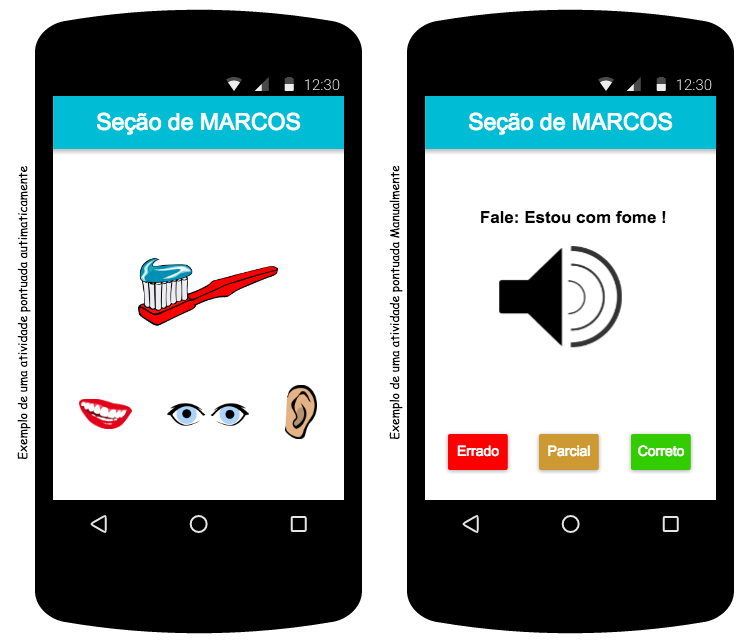
\includegraphics[scale=0.6]{img/integracaopaciente.png}
			\caption{Protótipo da Telas de Integração}
			Fonte:Autor, 2018
			\label{integracao}
		\end{figure}
		
		A imagem acima, Figura \ref{integracao}, mostra as telas nas quais o paciente estará em contato diretamente, essas precisam ser atraentes e auto explicativas para que o paciente consiga interagir fluidamente com o aplicativo.
		
		\subitem3 - Engajamento: é a forma de fazer com que o paciente queira ficar no jogo, no caso do aplicativo, será com o oferecimento de recompensas, como: mini games e mini clipes, realizar uma atividade de forma correta. Isso irá incentivar o paciente a resolver o que lhe for proposto de maneira correta, para que com isso receba a recompensa. Para que o paciente se sinta engajado a permanecer no jogo, é preciso que o mesmo tenha um visual atraente em relação a faixa etária, levando em consideração também a patologia do paciente.
		
		\begin{figure}[H]
			\centering
			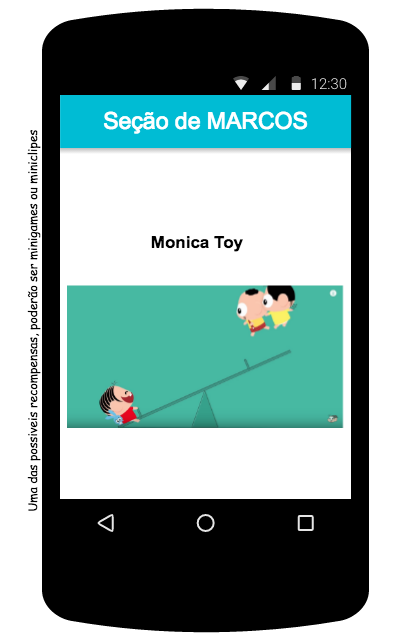
\includegraphics[scale=0.6]{img/pacienteengajamento.png}
			\caption{Protótipo da Tela de Bonificação}
			Fonte:Autor, 2018
			\label{engajamento}
		\end{figure}
	
		A Figura \ref{engajamento} mostra a bonificação recebida pelo jogador/paciente ao responder uma atividade de forma correta, podendo esta ser um vídeo, um mini game ou uma mini história em áudio. Esse tipo de bonificação é necessário para manter o engajamento do paciente no ambiente gamificado, ou seja, se trata de um estímulo ao uso do aplicativo.
		
	\item Mecânicas relacionadas aos responsáveis
		\subitem1-Desafios:  os desafios servem para estimular os pais ou responsáveis à acompanhem o tratamento dos filhos através da aplicação. Dessa forma eles poderão ajudar e apoiar seu filho em atividades extras, dado um suporte adicional no aprendizado das atividades propostas.
		
		\begin{figure}[H]
			\centering
			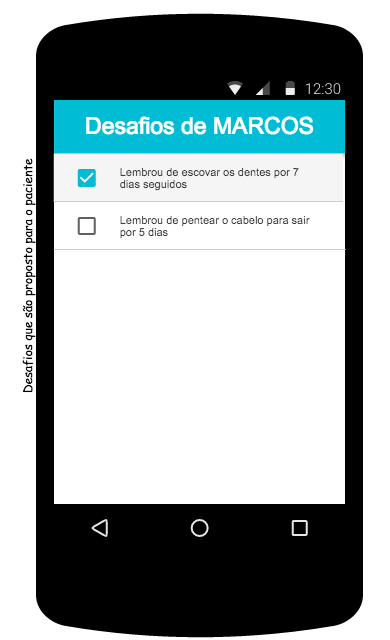
\includegraphics[scale=0.6]{img/desafiosparaopaciente.png}
			\caption{Protótipo da Tela de Desafios do Pacientes}
			Fonte:Autor, 2018
			\label{desafios}
		\end{figure}
		
		A imagem acima, Figura \ref{desafios}, mostra os desafios que a criança deve cumprir. Cada desafio deve ser analisado e respondido pelo responsável, gerando um comprometimento da evolução da criança. Com a conclusão de cada desafio, o paciente receberá uma recompensa.
		
		\subitem2 - Pontos: os pontos servem para que os pais possam acompanhar a evolução e desenvolvimento do filho. É uma maneira bem clara de  demonstrar o avanço através do uso da aplicação. Os pontos serão contabilizados de acordo com as atividades que o paciente realizar no aplicativo, e esses serão dados dependendo do nível da atividade que ele realizar, ou seja, a pontuação se trata de um \textit{feedback} quantitativo sobre o tratamento que está sendo realizado.
		
		\begin{figure}[H]
			\centering
			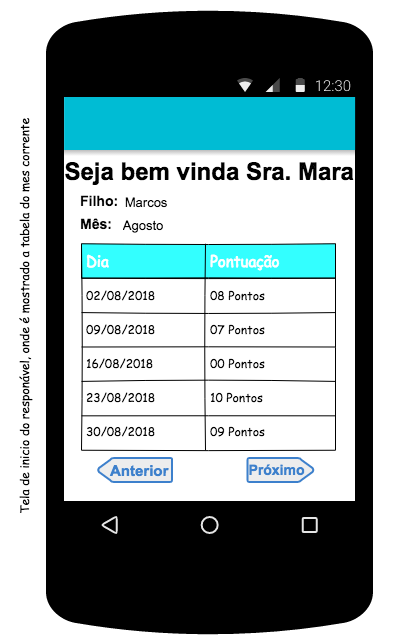
\includegraphics[scale=0.6]{img/pontospaciente.png}
			\caption{Protótipo da Tela Pontuação do Paciente para o Responsável}
			Fonte:Autor, 2018
			\label{pontos}
		\end{figure}
		
		A Figura  \ref{pontos} acima, apresenta a tela em que os responsáveis poderão visualizar o desempenho do seu filho no decorrer das sessões. A tela exibe uma tabela onde fica amostra as datas e pontuações feitas pelo paciente em um determinado mês.
		 
		\subitem3 - Níveis: os níveis atuarão em conjunto dos pontos, para que os responsáveis consigam acompanhar a evolução do desenvolvimento do seu filho. A evolução dos níveis será através dos pontos alcançados por cada atividade concluída pelo paciente, ou seja, quanto mais atividade ele resolver, mais pontos serão computados e consequentemente a mudança de nível será alcançada. 
		\begin{figure}[H]
			\centering
			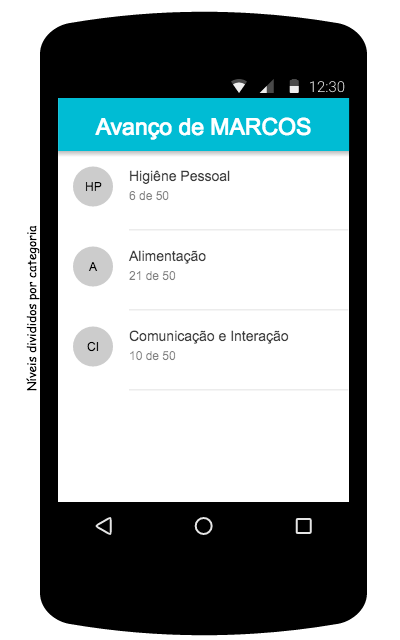
\includegraphics[scale=0.6]{img/niveisporcategoria.png}
			\caption{Protótipo da Tela de Níveis por Categoria}
			Fonte:Autor, 2018
			\label{niveis}
		\end{figure}
		A Figura \ref{niveis}  apresenta o protótipo da tela de níveis por categoria, cada categoria é composta por uma determinada quantidade de atividades, sendo que para avançar para outra atividade é necessário que o paciente responda corretamente as questões propostas.
		
	\item Mecânicas relacionadas aos profissionais
		\subitem1 - Pontos: para os profissionais, a pontuação serve para avaliar e acompanhar o desempenho de seus pacientes, dessa forma, através da pontuação, o profissional saberá se o paciente está indo bem ou mal nas seções de terapia. Os pontos servem também como um \textit{feedback} quantitativo sobre o tratamento que está sendo realizado com cada paciente, sendo possível ver a pontuação individual e também a pontuação geral em formato de ranking.
		
		\begin{figure}[H]
			\centering
			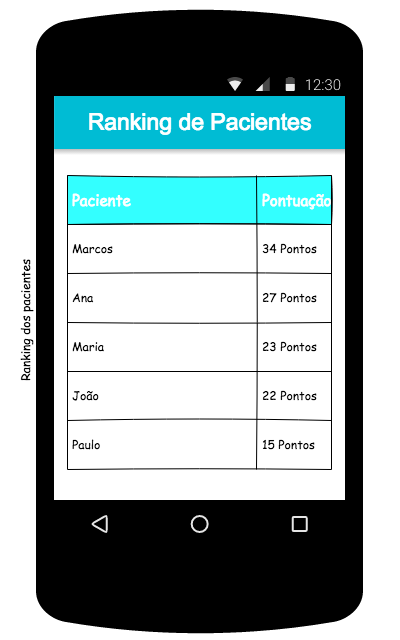
\includegraphics[scale=0.6]{img/rankingpaciente.png}
			\caption{Protótipo da Tela de Ranking de Pacientes}
			Fonte:Autor, 2018
			\label{ranking}
		\end{figure}
		
		A imagem acima, Figura \ref{ranking}, mostra a tela de pontuação em formato de ranking,  esses pontos servem para o profissional avaliar, por exemplo, como o paciente esta se desenvolvendo como uso da ferramenta.
		
		\subitem2 - Níveis: assim como para os responsáveis, os níveis servem para que o profissional possa acompanhar a evolução de seu paciente e saber como ele está se desenvolvendo com o uso da aplicação. O aplicativo irá aumentar os níveis de dificuldade gradativamente, ou seja, a cada mudança de nível, a atividade fica mais complexa e mais difícil de se realizar.  A Figura \ref{niveis} representa a tela de nível de um determinado paciente.
		
		
		\subitem3 - Classificação: a classificação serve para que o profissional consiga verificar a evolução de todos os seus pacientes em uma única tabela e, assim, apurar qual tem um melhor avanço nos tratamentos, bem como, qual paciente precisa de uma atenção maior por não estar correspondendo tão bem ao tratamento.
	
     	A Figura \ref{ranking}, mostra a tela onde serão classificados os pacientes do profissional, de acordo com a pontuação em ordem decrescente.
\end{itemize}

\section{Artefatos do Projeto de Software}
Está seção apresentará os fragmentos de diagrama de classe do núcleo do sistema, que abrange os principais casos de uso, os artefatos completos podem ser observados nos apêndices.
\begin{figure}[H]
	\centering
	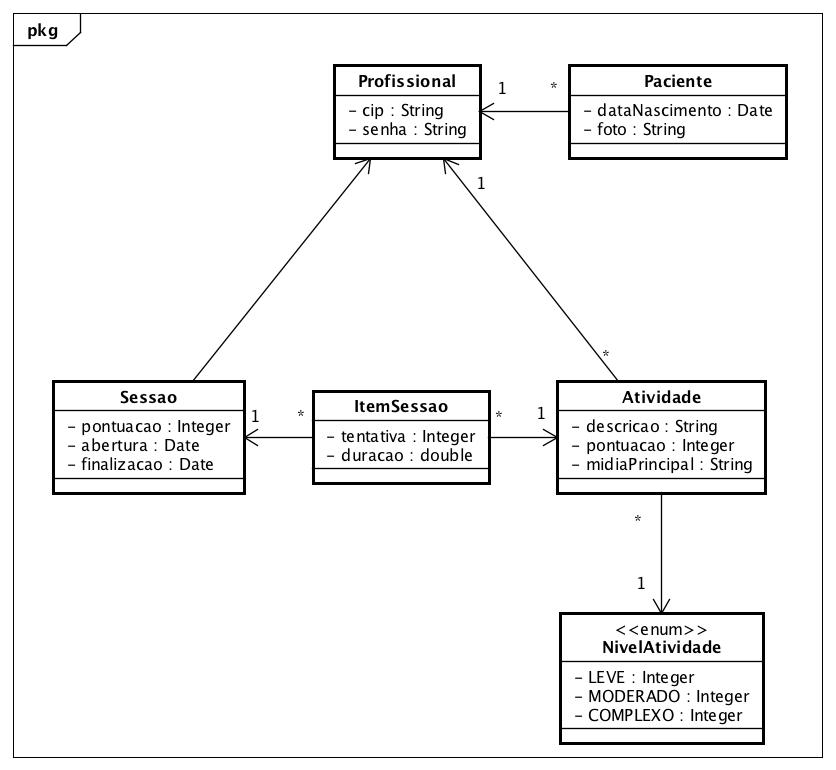
\includegraphics[scale=0.5]{img/UC_ControlarSessao1.jpg}
	\caption{Classes para UC Controlar Sessão - Parte 1}
	\label{pt1UC1}
	Fonte:Autor, 2018
\end{figure}
A Figura \ref{pt1UC1} representa no diagrama de classes a parte do caso de uso definido como Controlar sessões, de acordo com  o diagrama, o profissional deve realizar o cadastro das atividades que serão realizadas pela criança, classificando-as de acordo com o nível, essa informação será importante na hora de escolher qual atividade selecionar para a criança,tendo isso feito, ele deve escolher um paciente no inicio do aplicativo para iniciar a sessão, com isso ela se inicia,com isso pronto o paciente poderá repetir cada atividade um indeterminado número de vezes, por fim, quando o paciente terminar a pontuação final é gravada.

\begin{figure}[H]
	\centering
	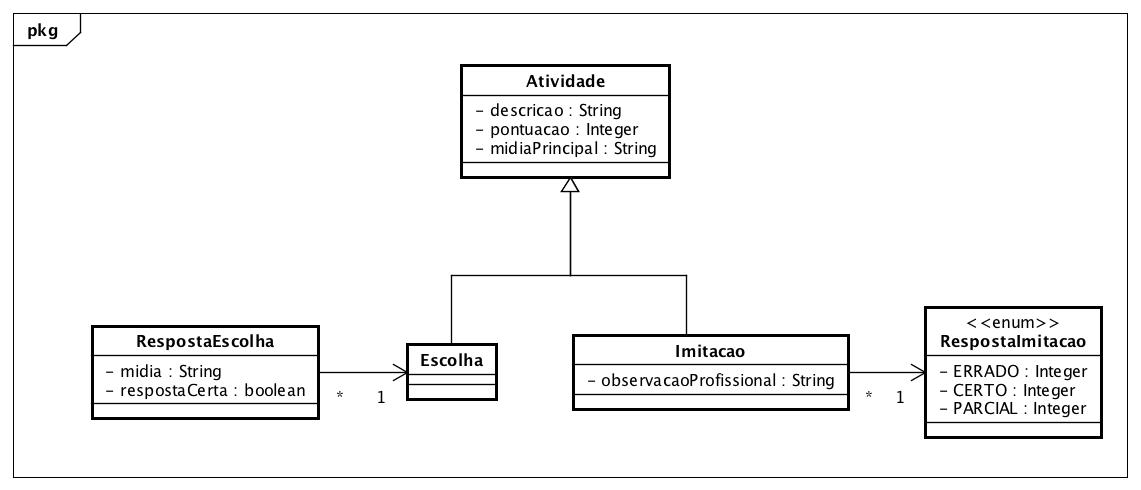
\includegraphics[scale=0.4]{img/UC_ControlarSessao2.jpg}
	\caption{Classes para UC Controlar Sessão - Parte 2}
		\label{pt2UC1}
	Fonte:Autor, 2018
\end{figure}
A Figura \ref{pt2UC1}, é a segunda parte  no diagrama de classes onde é definido o caso de uso Controlar sessão, de acordo com o diagrama, o aplicativo irá ofertar dois tipos de atividades, as de escolha e as de repetição.

\begin{figure}[H]
	\centering
	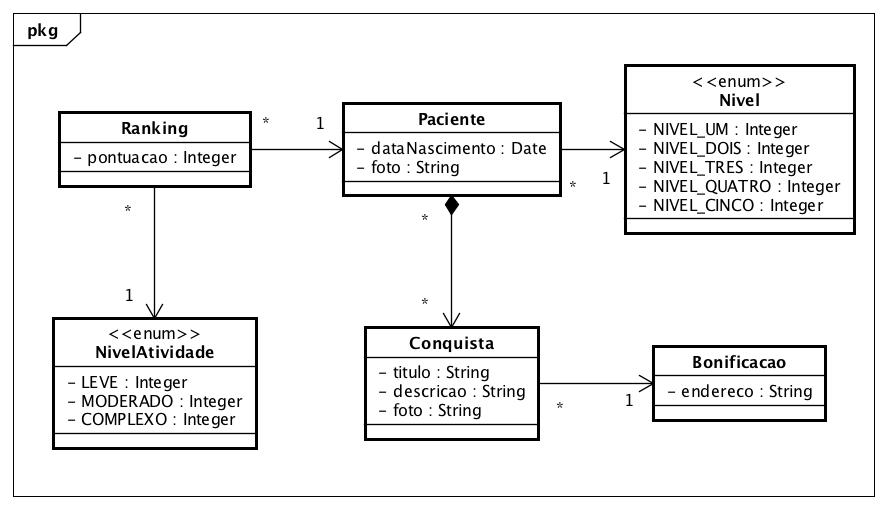
\includegraphics[scale=0.5]{img/UC_ControlarSessao3.jpg}
	\caption{Classes para UC Controlar Sessão - Parte 3}
		\label{pt3UC1}
	Fonte:Autor, 2018
\end{figure}
A Figura \ref{pt3UC1} demonstra ainda classes que fazer parte do caso de uso Controlar sessão, tendo ele a parte onde é montado o ranking do paciente pegando a pontuação, e consequentemente o nível de atividade que aquele paciente consegue resolver. É demonstrado que ele tem uma lista de conquistas que geram para ele uma bonificação.

\begin{figure}[H]
	\centering
	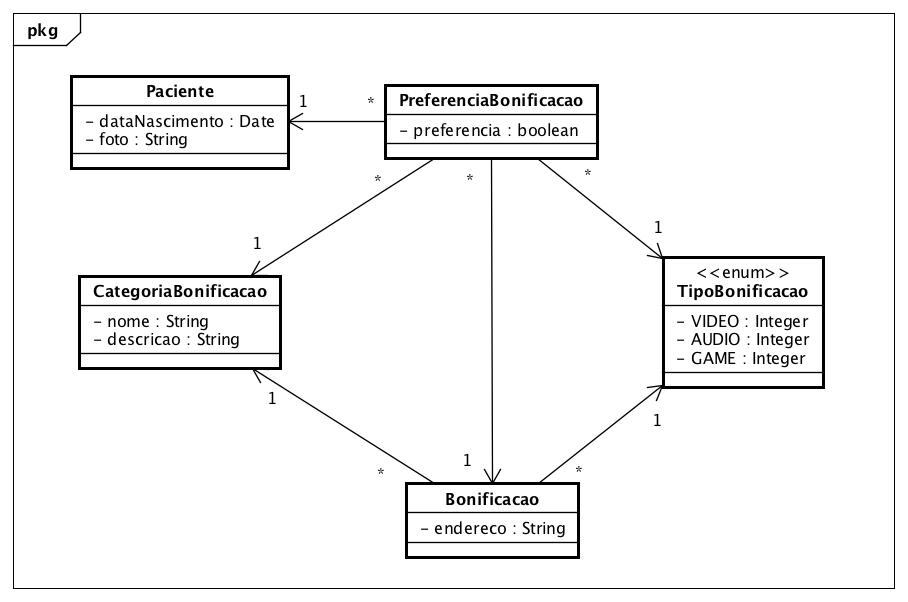
\includegraphics[scale=0.5]{img/UC_ControlarPreferenciasDeBonificacao.jpg}
	\caption{Classes para UC Controlar Preferencia da Bonificação}
		\label{pt1UC2}
	Fonte:Autor, 2018
\end{figure}
No fragmento do diagrama de classe mostrado na Figura \ref{pt1UC2}, são demonstradas as classes que representam a parte do caso de uso de controlar preferencias da bonificação, sendo que para cada paciente pode-se escolher preferencias para as bonificações que serão ofertadas a ela após concluir uma atividade com exito ou conseguir uma conquista, essas preferencias podem ser definidas pela categoria da bonificação, como por exemplo: Circo, mar, zoológico, pre-histórico, dentre outras preferencias ou pelo tipo da bonificação, que pode ser: vídeo, áudio ou um mini game. Após a excursa desses filtros, é trazido ao paciente aquela bonificação através da URI de localização dela.

\section{Considerações Finais}
Este capítulo apresentou os resultados obtidos durante este trabalho, que foram as relação de mecânicas de gamificação por atores do sistema, e os artefatos que irão compor o núcleo principal do sistema. Foram produzidos artefatos como: diagrama de casos de uso, diagrama de classes, protótipos e especificação de requisitos se encontram nos apêndices do trabalho.